Next, we switch to the MISO case and investigate the influence of transmit antenna (Tx) on the R-E region. The same multipath channel model is assumed in the simulation. Thanks to the decoupling approach, the predetermined beamforming phases ${\mathbf{\Phi }}_I^ \star ,{\mathbf{\Phi }}_P^ \star $ are optimal for MISO and the computational complexity is irrelevant to $M$. Figure \label{fig:miso-re-instance} shows the result over an instance FF channel for $M = 2,3$ and $N = 4$.

\begin{figure}[ht]
  \centering
  \subfigure[Instance]{
    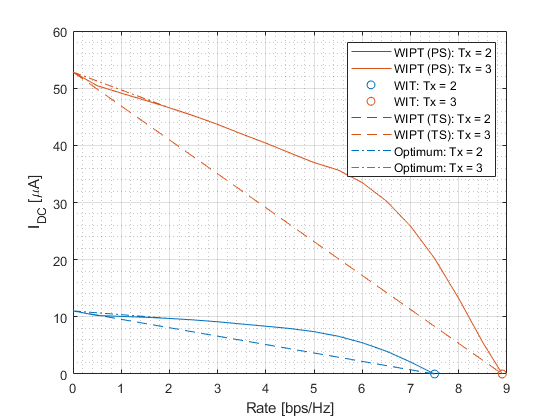
\includegraphics[width=0.48\textwidth]{miso_re_instance}\label{fig:miso-re-instance}}
  \subfigure[Average]{
    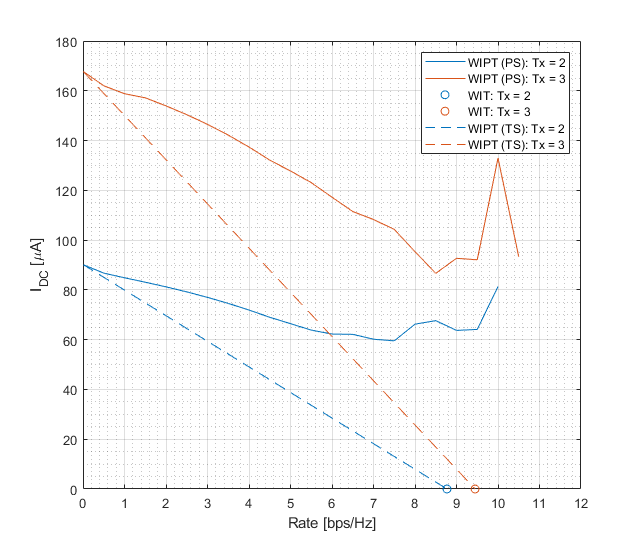
\includegraphics[width=0.48\textwidth]{miso_re_average}\label{fig:miso-re-average}}
  \caption{R-E region vs $M$ over FF channel: an instance and the average over 100 realizations}
  \label{fig:miso-re}
\end{figure} 

A first observation is that the concacity-convexity appears for $N = 4$ for the MISO systems, in contrast to $N = 8$ in the SISO case. It suggests that a large $M$ can further boost the energy benefit by multisine waveform. The reason is that increasing $M$ essentially produces more subchannels for transmission such that the coupled terms contributing to the harvested current are amplified. Also, a smaller $N$ is needed to achieve a certain output current level and the transmitted waveform is with a lower PAPR. Hence, increasing $M$ can be a possible solution for PAPR-constrained devices. Moreover, a combination of TS (between WPT and WIPT) at low rate and PS at high rate guarantees the optimal R-E region as a convex hull.

To eliminate the influence of channel randomness, we investigate the R-E tradeoff for 100 FF channels with $N = 4$. However, the averaged plot of Figure \ref{fig:miso-re-average} is not a good representation for the general performance. At the low-rate region ($R \leqslant 5$ bps/Hz), the curves showed some concacity as expected. This is because the capacity of most channels can satisfy such a low rate constraint and guarantee valid R-E pairs that contributes to the averaged points. Nevertheless, as the rate constraint increases, only strong channels can support WIPT while those weak channels are abandoned. For instance, if the per-subband rate requirement is 10 bps/Hz but the capacity of 90 \% channels are below this value, then only 10 \% channels will be considered in the averaging. Therefore, the high-rate region is indeed dominated by some strong channels. Increasing the number of channels may mitigate the phenomenon to some extent, but a better representation is required to avoid channel randomness and characterize the general R-E region.

Figure \ref{fig:miso-cdf} shows the Cumulative Distribution Function (CDF) of maximum rate and DC current that correspond to WIT and WPT respectively. It is less interesting for WIPT since the variation trend of the R-E tradeoff is not presented.

\begin{figure}[ht]
  \centering
  \subfigure[Rate]{
    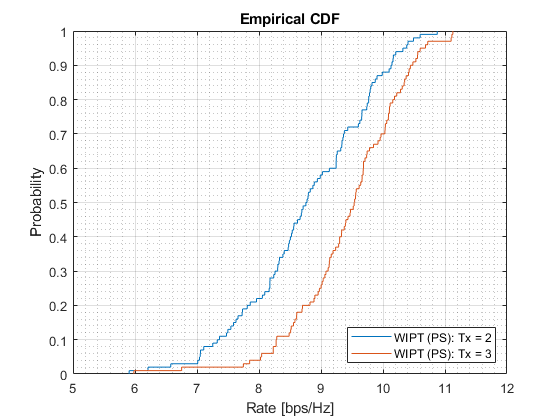
\includegraphics[width=0.48\textwidth]{miso_cdf_rate}\label{fig:miso-cdf-rate}}
  \subfigure[Current]{
    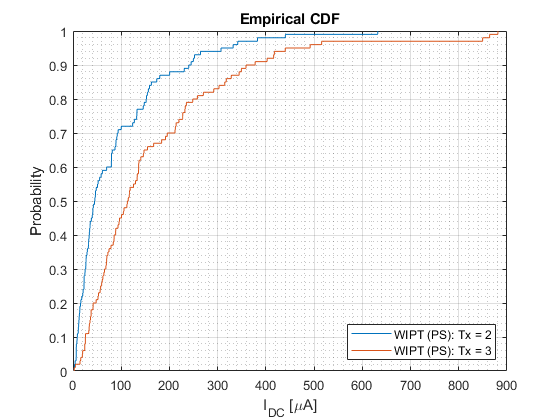
\includegraphics[width=0.48\textwidth]{miso_cdf_current}\label{fig:miso-cdf-current}}
  \caption{Rate and current CDF vs $M$ for MISO FF channels}
  \label{fig:miso-cdf}
\end{figure} 